\chapter{Implementation}\label{ch:implementation}
\section{Introduction}\label{sec:implementation:introduction}
Having the requirements specified, a project created, and tools chosen, the implementation phase may begin. Section \ref{sec:implementation:tools} will introduce the remaining tools used during the development. A package diagram presented in Section \ref{sec:implementation:architecture} will help depict the final high-level architecture of the system. Section \ref{sec:implementation:challenges} will describe challenges encountered during the implementation. The application installation and usage will be described in Section \ref{sec:implementation:installation} In the Summary (Section \ref{sec:implementation:summary}), the implementation phase and its steps will be summarized.

\section{Development Environments and Tools}\label{sec:implementation:tools}
In addition to the tools mentioned in Chapter \ref{ch:tools}, various development environments and tools were used. They will be briefly described in this section.

\subsection{Android Studio}
\textit{Android Studio}\footnote{https://developer.android.com/studio (accessed Dec. 12, 2020)} is the official IDE (\textit{Integrated Development Environment}) for Android development. Since the Flutter release, it also supports this framework (only compilation to Android). It provides an extensive functionality - from standard code editor, through debugging tools, to device emulators. Because it is a project derived from the IntelliJ IDEA Community Edition\footnote{https://www.jetbrains.com/idea (accessed Dec. 12, 2020)}, it is distributed under an Apache 2 license\footnote{https://www.apache.org/licenses/LICENSE-2.0 (accessed Dec. 12, 2020}), which is an open-source license and allows for development within the needs of the project.


\subsection{Flutter console}
Flutter console allows for the Flutter application development management. The most used commands are:
\begin{itemize}
    \item \texttt{flutter analyze} - performs a static code analysis.
    \item \texttt{flutter build} - builds the application.
    \item \texttt{flutter doctor} - shows information about the installed tooling and allows to detect issues.
    \item \texttt{flutter pub} - allows for Flutter packages management.
    \item \texttt{flutter run} - runs the Flutter application on an attached device (allows for running, controlling and debugging multiple devices at a time).
\end{itemize}
Whilst it is possible to run most of them through the IDE, it is more convenient to do it from the terminal (especially if performed often).


\section{High-Level Architecture Overview}\label{sec:implementation:architecture}
Flutter's projects structure (high level of modularity and numerous classes related to the view layer of the application) causes the class diagram to be overcomplicated. The deployment diagram would be relatively similar to the basic architecture diagram presented in Section \ref{subsec:tools:architecture:basic}. However, it is not detailed enough to provide a comprehensive overview of the implemented system. In order to illustrate the high-level architecture of the application, a simplified package diagram was created and is presented in Figure~\ref{fig:diagrams:package-diagram}.
\\
\begin{figure}[htb]
\centering
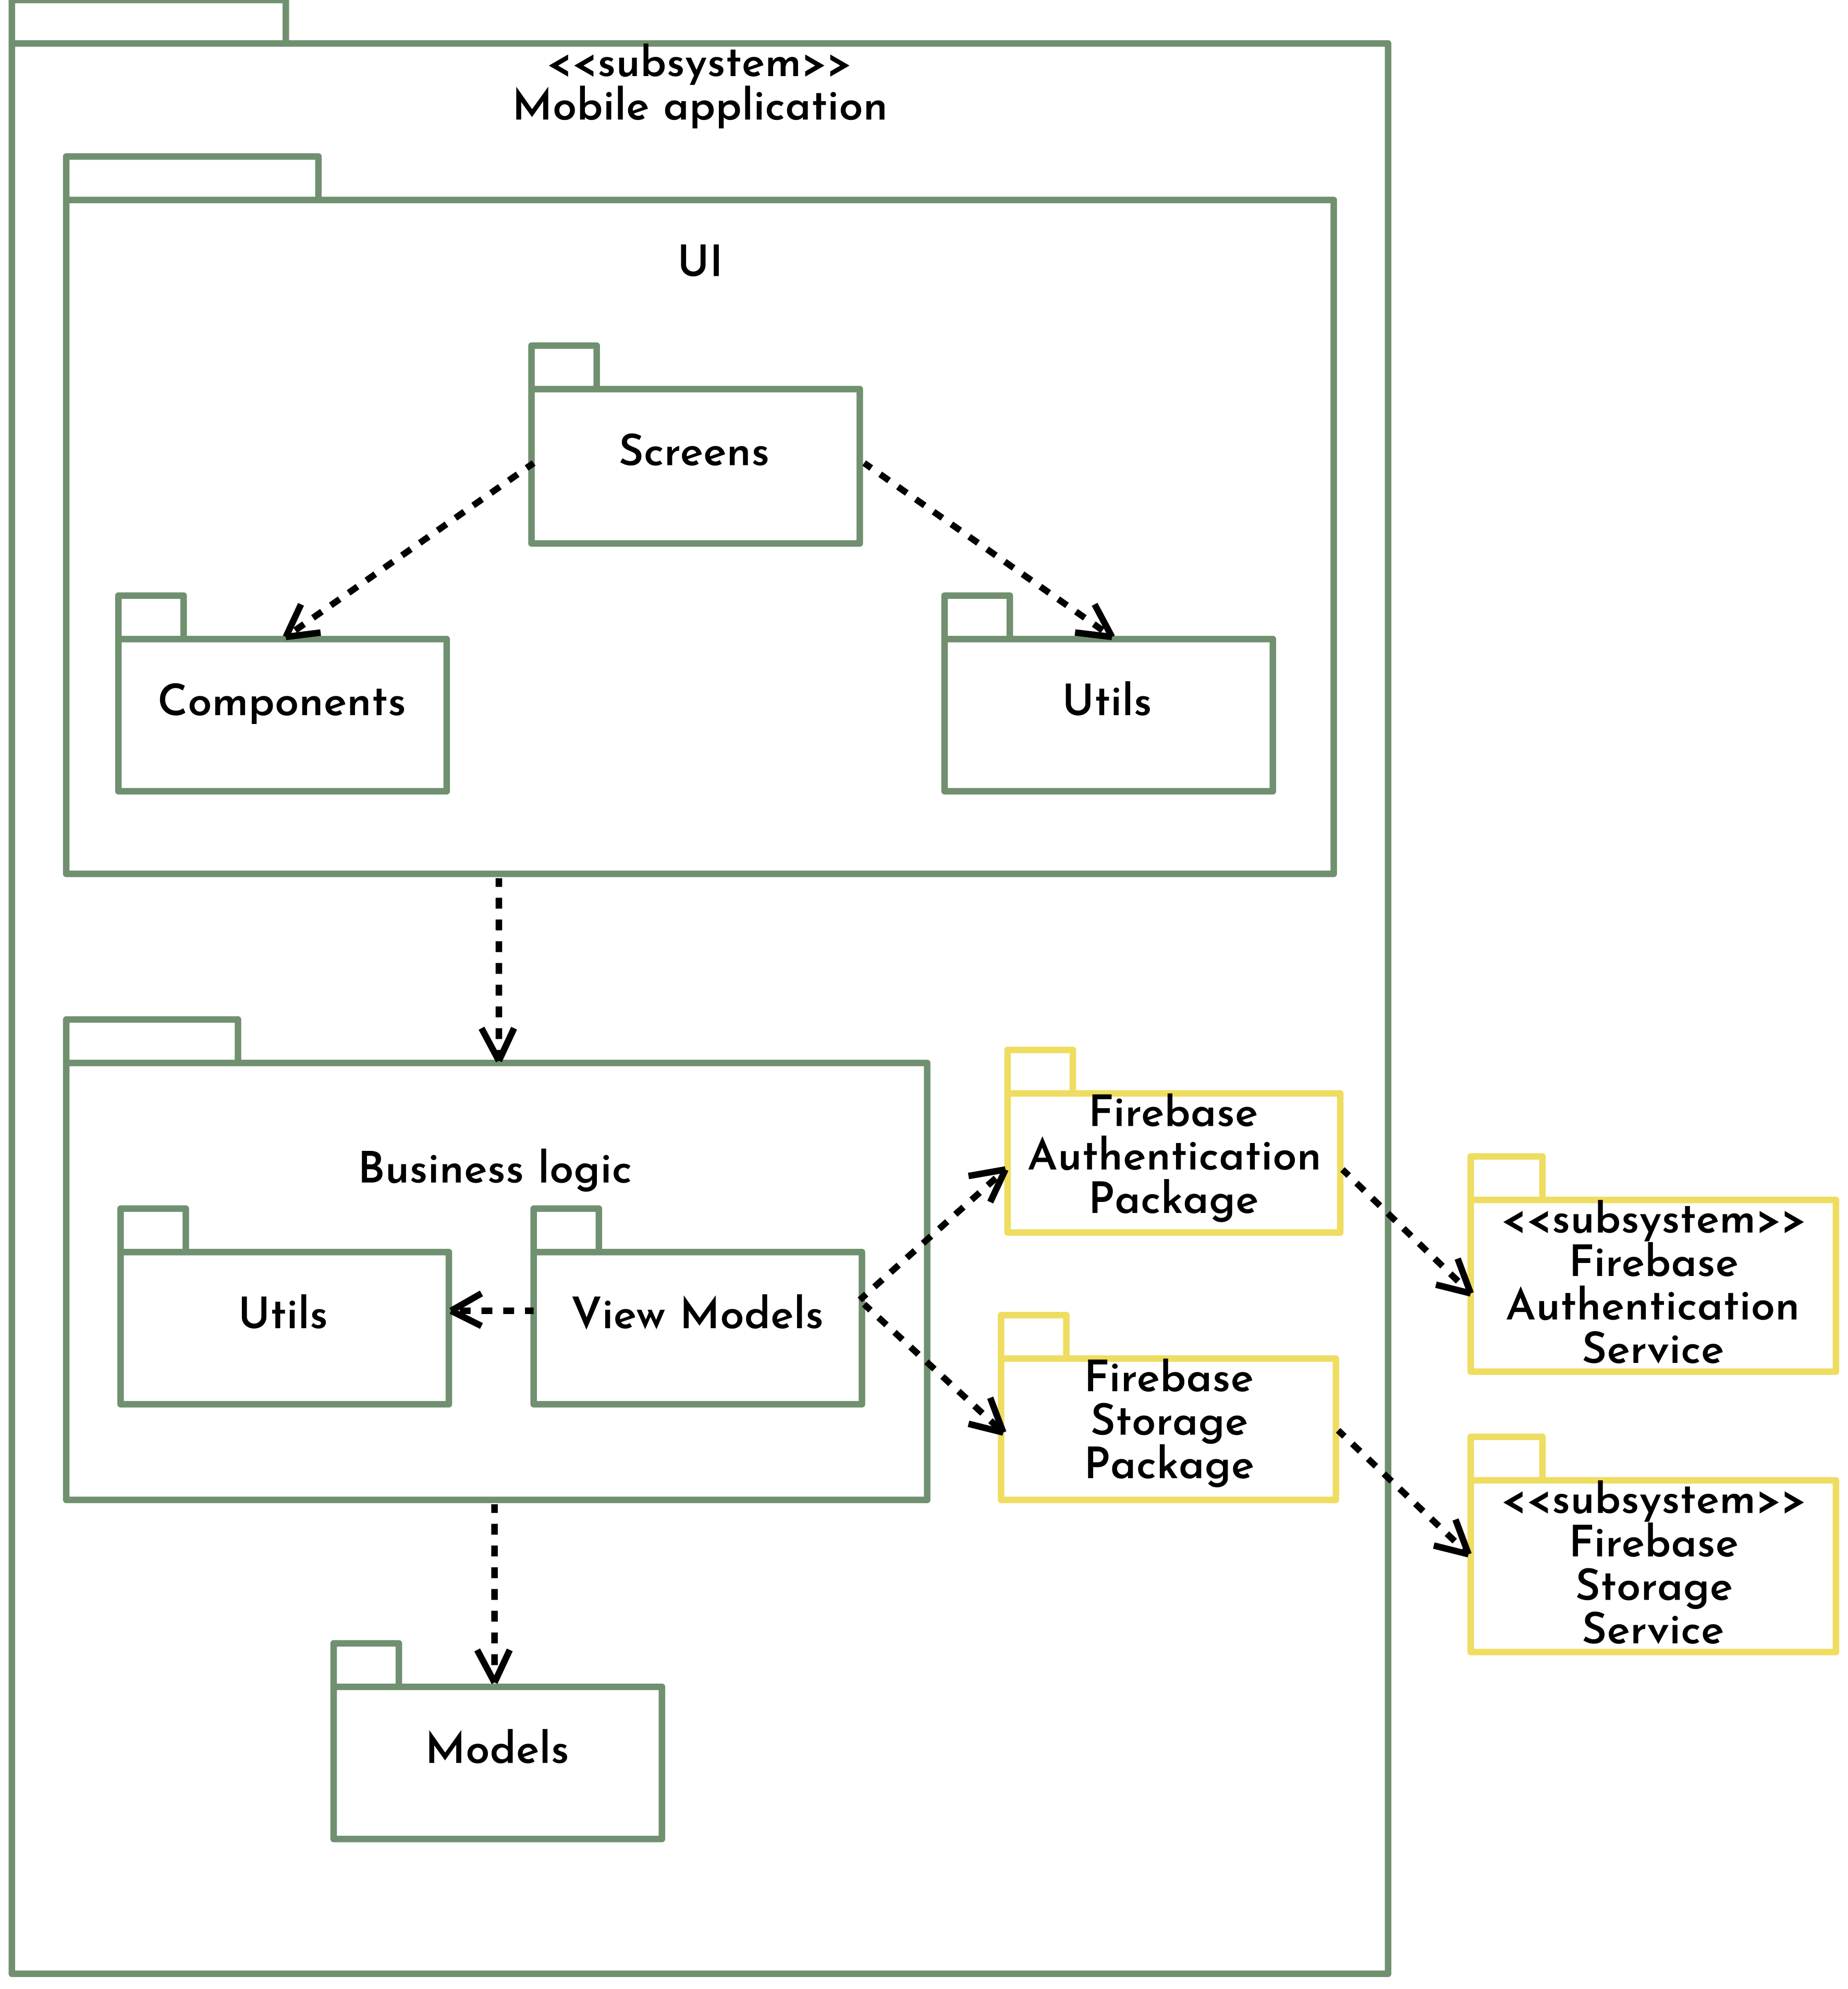
\includegraphics[width=.9\linewidth]{images/diagrams/package-diagram.png}
\caption{A simplified package diagram of the implemented system}
\label{fig:diagrams:package-diagram}
\end{figure}
\\
The mobile application, following the MVVM design pattern, was divided into 3 main packages.
\\\\
UI (\textit{User Interface}) consists of three packages. \textit{Screens} package contains application screen classes (i.e. \texttt{LoginScreen} or \texttt{RewardsScreen}). \textit{Components} are classes that are reused (at least twice) in within the \textit{Screens} package. \textit{Utils} package contains functions responsible for displaying modal windows.
\\\\ 
\textit{Business logic} package consists of the \textit{Utils} (which plays a similar role as in the \textit{UI} package) and \textit{View Models} packages. View models depend on two packages that allow for communication with services. If the services were implemented in a traditional manner, they would be a part of the \textit{Business logic}, however, to emphasize their independence, they were depicted separately. Both service packages depend on the service subsystems.
\\\\
\textit{Models} package contains models (such as \textit{task}, \textit{child}, \textit{parent} or \textit{reward}) and enumerations (application login state or device belonging).


\section{Implementation challenges}\label{sec:implementation:challenges}
Every project has its challenges. Ideally, they should be detected and prevented (or at least minimize their impact). Reality, however, is never ideal. It is important to identify those challenges and draw conclusions from them. The latter will be done in the Chapter \ref{ch:summary}, the former will be described in this section.


\subsection{User Interface}
Many custom, atypical user interface elements, especially the header, could not be implemented using standard techniques. These assume the customisation of the \texttt{AppBar}\footnote{https://api.flutter.dev/flutter/material/AppBar-class.html (accessed Dec. 13, 2020)}widget, or, in more complicated cases, \texttt{SliverAppBar}\footnote{https://api.flutter.dev/flutter/material/SliverAppBar-class.html (accessed Dec. 13, 2020)}. Due to the complexity of the user interface visuals, a \texttt{Canvas}\footnote{https://api.flutter.dev/flutter/dart-ui/Canvas-class.html (accessed Dec. 13, 2020)} class was used.
\\\\
The \texttt{Canvas} class is an interface for recording graphical operations. While being much more complex than other widgets, provides a higher flexibility and control over its visual output. 
\\\\
It was used to implement the header, along with the footer, but not without difficulties. During the development, issues with interoperability with other widgets emerged. Its initially infinite clip region, repeatedly caused problems with overlapping or being overlapped by other components. Another vital problem emerged during the header title implementation. Text on Canvas, instead of being an embedded \texttt{Text}\footnote{https://api.flutter.dev/flutter/dart-html/Text-class.html (accessed Dec. 13, 2020)} widget, needs to be rendered by a \texttt{TextPainter}\footnote{https://api.flutter.dev/flutter/painting/TextPainter-class.html (accessed Dec. 13, 2020)} class. It caused less control over how the text is displayed.


\subsection{Provider}
State management using \texttt{Provider} and the reasons for its adoption have been described in Section \ref{subsec:tools:architecture:state}. During the implementation, with increasing number of Provider classes, their maintenance had started to become slightly cumbersome and ineffective. In the final implementation there are 11 different Provider classes implemented and would increase, in case of the application growth.
\\\\
Additionally, sometimes Providers depend on one another. This enforces a usage of \texttt{ProxyProviders}, which take other Providers as a constructor argument. A dependency created this way, causes even more complication and boilerplate code.

\section{Installation}\label{sec:implementation:installation}
The development project has been built into a \texttt{raise-app.apk} android package file and is attached with this document (in order to install the application from outside of the Google Play platform, special permissions might be required).
\\\\
The newest version, however, can be found on the Google Play platform under \href{https://play.google.com/store/apps/details?id=dev.karbownik.raisef\_app}{this link}\footnote{https://play.google.com/store/apps/details?id=dev.karbownik.raise\_app (accessed Dec. 14, 2020)}.

\section{Summary}\label{sec:implementation:summary}
Over the course of the implementation phase, a full application planned during the previous phases has been completed. Thanks to the project phase, where the application was planned, and despite occasional challenges that occurred, the process has been finished with a product that is ready for the end-user testing and release.